% Exemplo de beamer
% Para compilar siga a ordem: pdflatex -> bibtex -> pdflatex -> pdflatex
% author: Bruno Normande
%
% tipo de documento tem que ser "beamer" para fazer apresentação
\documentclass[11pt]{beamer}

% Alguns pacotes interessantes
\usepackage[utf8]{inputenc}
\usepackage[portuguese]{babel}
\usepackage{natbib}
\usepackage{url}
\usepackage{cite}
\usepackage[T1]{fontenc}
\usepackage{graphicx,subfigure}

% Existem várias combinações de temas e cores
% para vê-los: http://www.hartwork.org/beamer-theme-matrix/
\usetheme{Madrid}
\usecolortheme{beaver}

%isso aqui é para evitar um erro
% não sei exatamente para que serve hehe
\def\newblock{}

% título autor e datas serão formatados
% automaticamente quando usar o comando \maketitle
\title{Um Exemplo de Apresentação}
\author[Bruno N. Lins]{Bruno Normande Lins}
\date{\today}

% Marca o início do documento
\begin{document}

	% Esse frame inicial contém o título ;D
	\begin{frame}{}
		\maketitle
	\end{frame}
	
	% Esse comando inclui no começo de cada sessão o Roteiro da apresentação
	\AtBeginSection[]{
		\begin{frame}[<+-| alert@+>]{Roteiro da Apresentação}
			\small
			\tableofcontents[current,currentsection]
		\end{frame}
	}
	
	% Agora começa de verdade %%%%%%%%%%%%%%%%%%%%%%%%%%%%%%%%%%%%%%%%%%%%%%%%%%%%%%%%%%%%%%%%%%%%%%%%%%%%%%%%%%%%%%%%%%%%%
	%%%%%%%%%%%%%%%%%%%%%%%%%%%%%%%%%%%%%%%%%%%%%%%%%%%%%%%%%%%%%%%%%%%%%%%%%%%%%%%%%%%%%%%%%%%%%%%%%%%%%%%%%%%%%%%%%%%%%%%
	% Toda section é indexada automaticamente
	\section{Primeira sessão}
	
	\begin{frame}{Aqui fica o título do frame}
	
		\begin{block}{Título do block}
			Isso é um um block ;D
		\end{block}
		
		E aqui um texto sem bloco
		
		\begin{center}
			posso pôr também centralizado...
		\end{center}
		
		\hfill Ou alinhado à direita	
		
	\end{frame}
	
	\subsection{Também podemos pôr sub-sessões}

		\begin{frame}{}
	
		\begin{block}{}
			Nem o frame nem o block precisam necessariamente de títulos
		\end{block}
		
		% Divide o frame fazendo uma "pausa dramática"
		\pause 
		\begin{alertblock}{}
			\hfill O alertblock é um block de cor diferente
		\end{alertblock}
		
		%espaçamento vertical
		\vspace{1.5cm}
		;D isso está um pouco mais abaixo =x			
		
	\end{frame}
	
	\subsection{Itemize e Enumerate}
	\begin{frame}
		\begin{itemize}
			\item um item
			\item outro item
			\item e assim por diante...
		\end{itemize}
		\begin{enumerate}
			\item aqui ele enumera
			\item e você pode combinar
			\begin{itemize}
				\item existem várias possibilidades
				\begin{itemize}
					\item legal né?
				\end{itemize}
			\end{itemize}
		\end{enumerate}
	\end{frame}
	
	\section{Imagens e tabelas}
	
	\begin{frame}{Vamos pôr uma imagem agora}	
		% usamos o ambiente 'figure' pq ele já faz várias coisas automaticamente
		\begin{figure}
			\centering %como centralizar
			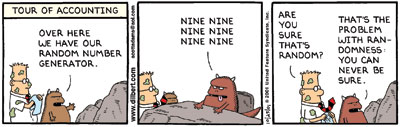
\includegraphics[width=0.5\linewidth]{random.jpg} % defino o width = metade do width de um linha
			\caption{``Random Numbers'' \citep{dilbert}} % na figure podemos por uma legenda - e aproveito para mostrar como fazer aspas e como citar algo da blibografia ;D			
			\label{fig:random} % posso atribuir um label para usar como referencia
			% btw: label tem que vir depois de caption, senão dá pau
		\end{figure}		
		E aqui uma referência a figura \ref{fig:random} % note que a numeração é automática
	\end{frame}
	
	\begin{frame}{E Uma Tabela Simples}	
		% Também podemos pôr a tabela dentro do ambiente table que funciona como o
		% ambiente figure, mas para tabela - a tabela em sí é feita com o ambiente tabular
		\begin{table}
			\centering
			% Ao começar uma tabela vc diz quantas colunas você quer
			% e qual a formatação delas (c = centralizado, r = direita...
			% e tem algumas outras)
			% se quisermos linha entre as colunas separamos por |
			\begin{tabular}{|c|c r|} % note que são 3 colunas sendo que entre as duas ultimas não tem linha
				\hline % linha horizontal
				Item 1 & Item 2 & Item 3 \\ % '&' separa colunas e '\\' pula uma linha
				\hline
				Mais & Uma & linha \\
				e & a & ultima \\ % não pus \hline entre as duas ultimas
				\hline
			\end{tabular}
			\caption{Uma tabela} % na figure podemos por uma legenda - e aproveito para mostrar como fazer aspas ;D			
			\label{tab:tab1} % posso atribuir um label para usar como referencia
		\end{table}		
		E aqui uma referência a tabela \ref{tab:tab1} % note que a numeração é automática
	\end{frame}	

	\section{Referências}	
	% allowframebreaks faz com que o frame se divida automaticamente
	% se o conterúdo for grande d+
	\begin{frame}[allowframebreaks]{Referências}
		\bibliographystyle{plain} % existem vários estilos poss´iveis
		\bibliography{referencias} % não preciso por .bib		
	\end{frame}		
	
\end{document}
